\chapter{Results}
\label{chp:results} 

\section{Introduction}

This chapter presents how the robot and the supporting implementations were tested. Tests were performed on a simulated version of the robot and the real hardware. The software is inherently indifferent to weather the robot is simulated or real. However, it was still necessary to have some separate launch and configuration files for the simulated and hardware version. 

\section{Testplan}

The following tests will be carried out in the simulator, as well as in the real world. They will mainly focus on the navigation stack and \ac{RTAB-Map}. 

\begin{table}
	\centering
	\begin{tabular}{ p{3.5cm} | p{7cm} }
		\multicolumn{2}{c}{Supporting Functionality}\\
		\hline
		\textbf{Evaluate} & Description\\
		\hline
		\textbf{Mobile application, ''Robot Leash''} & Use the mobile application to manually steer the robot.\\
		\textbf{Operator Control Station} & Steer the robot from the \ac{OCS} while monitoring the robot through the live video stream. \\
		\hline
		\textbf{Motor controller on XMEGA A3BU} & Verify ability to command the wheels. Confirm that the vehicle stops when velocity commands from \ac{ROS} are absent.\\
		\hline
	\end{tabular}
	\caption{}
\end{table}

\begin{table}
	\centering
	\begin{tabular}{ p{2.5cm} | p{7cm} }
	\multicolumn{2}{c}{Core Functionality}\\
\hline
	\textbf{Evaluate} & Description\\
	\hline
	\textbf{Multi Session Mapping} & Verify that the robot can rediscover areas which have been mapped in a previous mapping session.\\
	\hline
	\textbf{Loop Closure Detection} & As a core functionality in \ac{RTAB-Map}, it is critical to evaluate the loop closure mechanism.\\
	\hline
	\textbf{Autonomous Navigation} & Perform a set of tests on the navigation stack. The tests should evaluate path planning with moving obstacles. Different parameters should be tested and evaluated. Observe how the robot handles narrow passages. Evaluate robustness of the navigation stack for this robot.\\
	\hline
	%\caption{}
	\end{tabular}
	\caption{}
\end{table}


\subsection{Supporting Functionality}

\section{Results}

\section{Simulation Results}

The system was tested 

\begin{figure}[p]
	\centering
	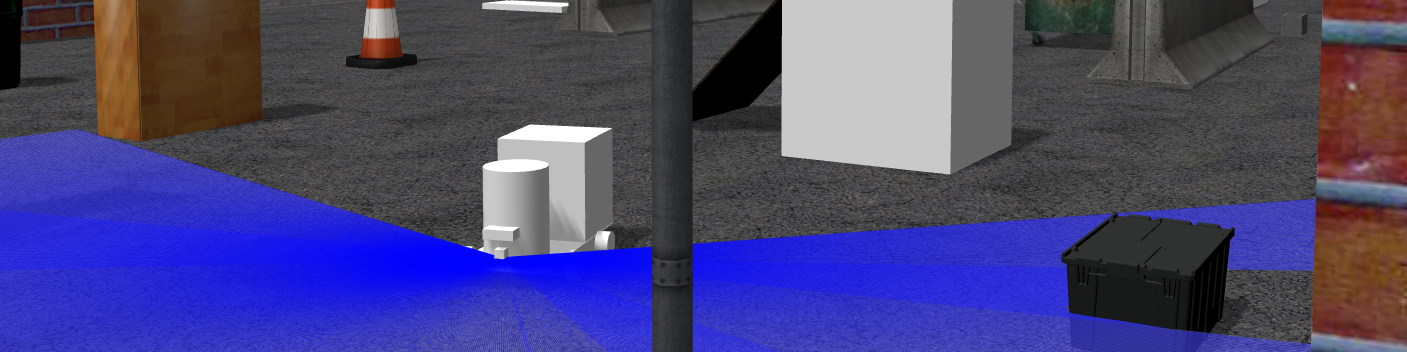
\includegraphics[width=1\textwidth]{gazebo2_cropped}
	\caption{The ''Asphalt'' world in Gazebo. }
	\label{fig:Incorrect_lc_detection}
\end{figure}

\begin{figure}[p]
	\centering
	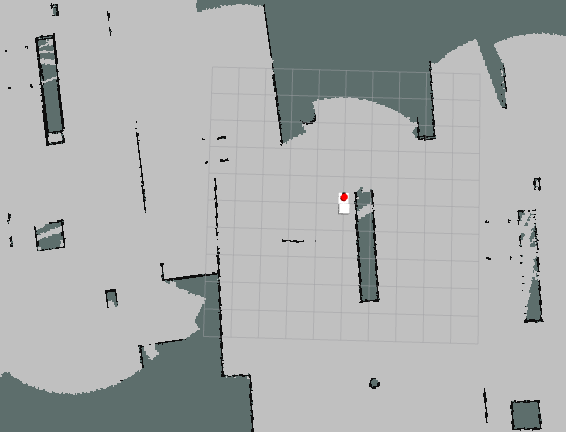
\includegraphics[width=1\textwidth]{Incorrect_lc_detection_cropped}
	\caption{An example of incorrect map merging. This case occurred in the ''Asphalt'' world simulated in Gazebo.}
	\label{fig:Incorrect_lc_detection}
\end{figure}

\begin{figure}[p]
	\centering
	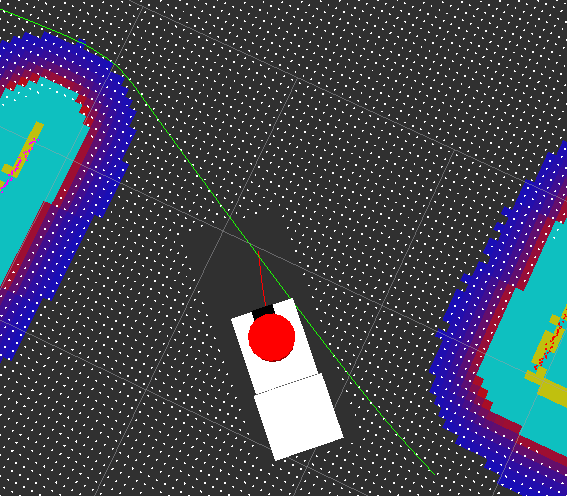
\includegraphics[width=1\textwidth]{planning_big_footprint_cropped}
	\caption{Nodes and topics for motion control. }
	\label{fig:big_footprint}
\end{figure}



\subsection{Live Testing}

Due to time constraints, it was no time to tune the parameters of \ac{RTAB-Map}.

\subsubsection{Safety Features}

\subsubsection{Loop Closure Detection}

\begin{figure}
	\centering
	\begin{subfigure}[b]{1\textwidth}
		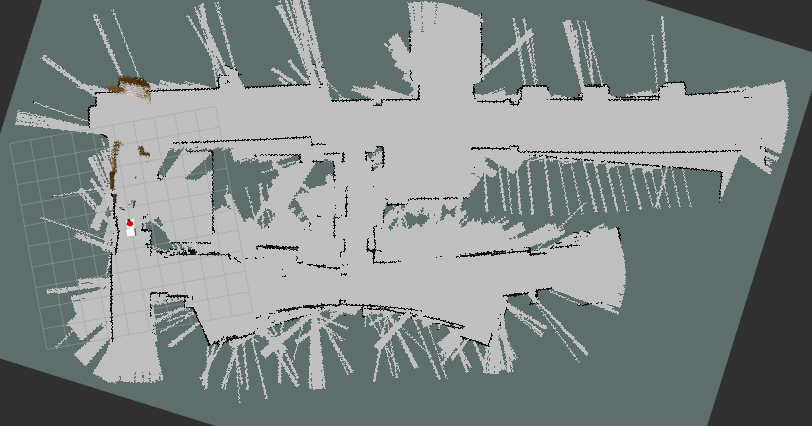
\includegraphics[width=\textwidth]{mapping_gamle_elektro}
		\caption{Resulting occupancy grid after a mapping session. The mapping  method is struggling with the  hallway in the upper part of the image.}
		\label{fig:mapping_gamle_elektro}
	\end{subfigure}
	\begin{subfigure}[b]{1\textwidth}
		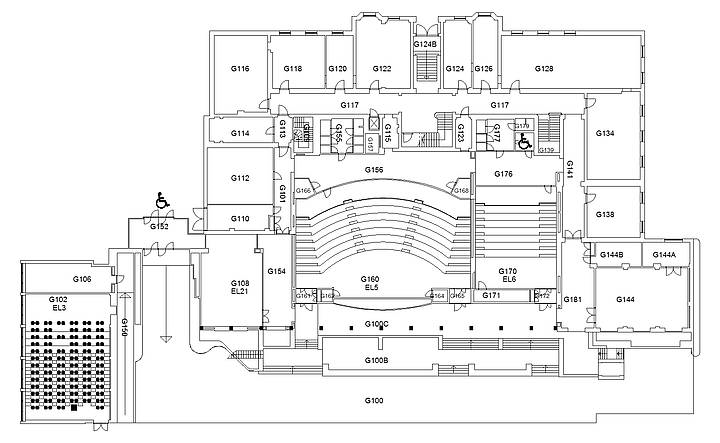
\includegraphics[width=\textwidth]{floorPlan}
		\caption{Floor plan of Gamle Elektro, first floor.}
		\label{fig:floorPlan}
	\end{subfigure}
	\caption{Comparison between mapped occupancy grid and floor plan.}
\end{figure}

\begin{figure}[p]
	\centering
	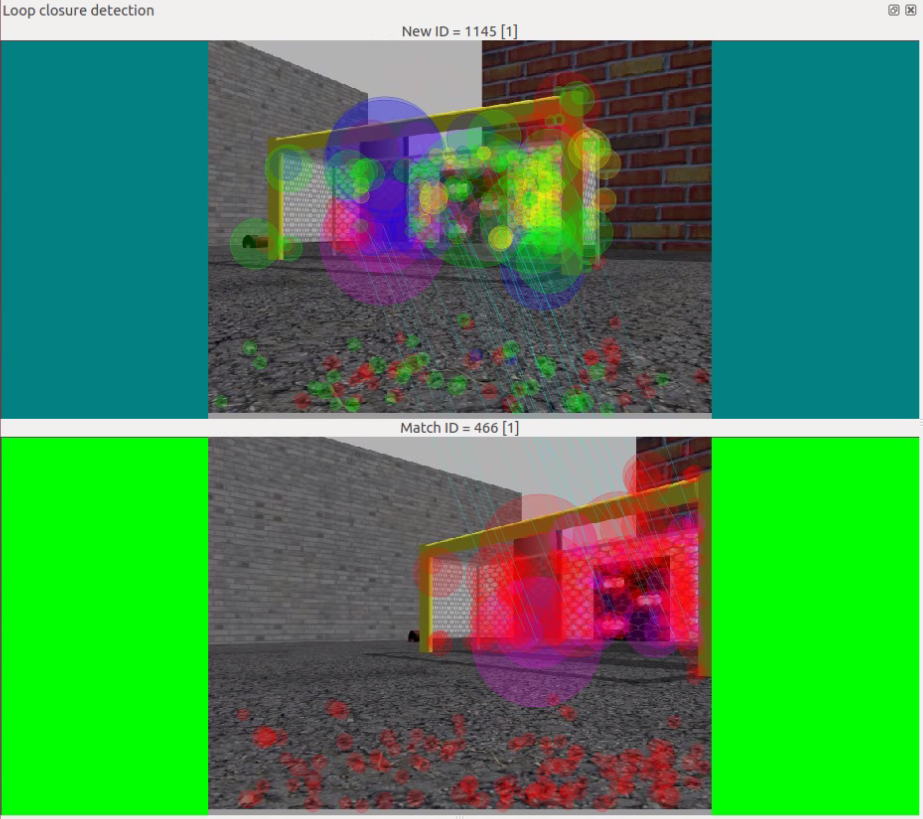
\includegraphics[width=1\textwidth]{loop_closure_detection}
	\caption{An example of an accepted loop closure hypothesis. This example is from the ''Asphalt'' world simulated in Gazebo.}
	\label{fig:loop_closure_detection}
\end{figure}

\begin{figure}[p]
	\centering
	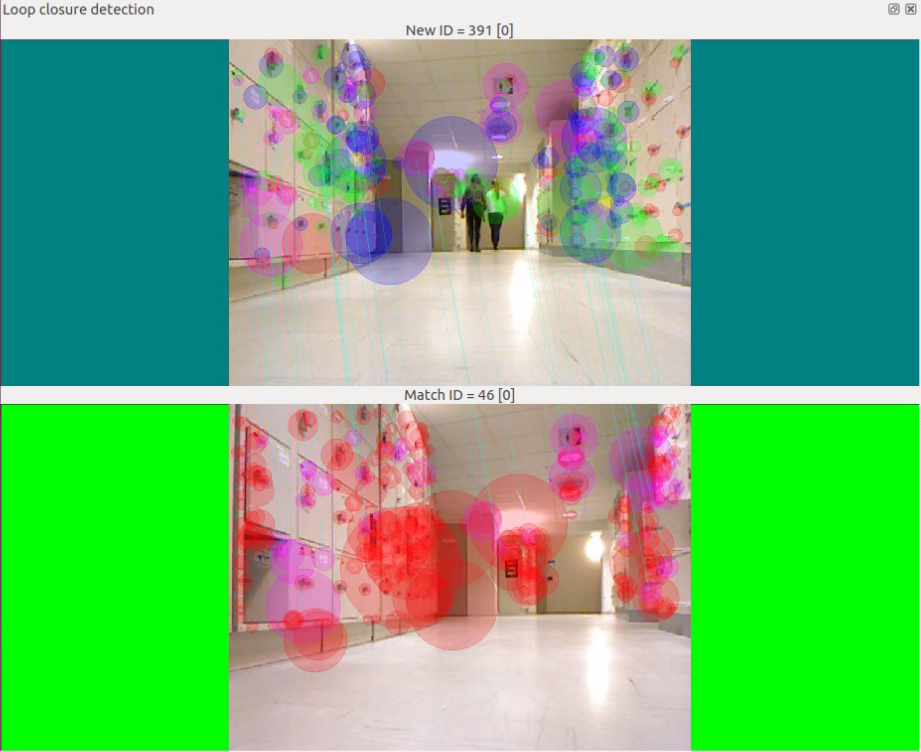
\includegraphics[width=1\textwidth]{lc_match_live}
	\caption{An example of an accepted loop closure hypothesis. This example is from the ''Asphalt'' world simulated in Gazebo.}
	\label{fig:lc_match_live}
\end{figure}

\begin{figure}[p]
	\centering
	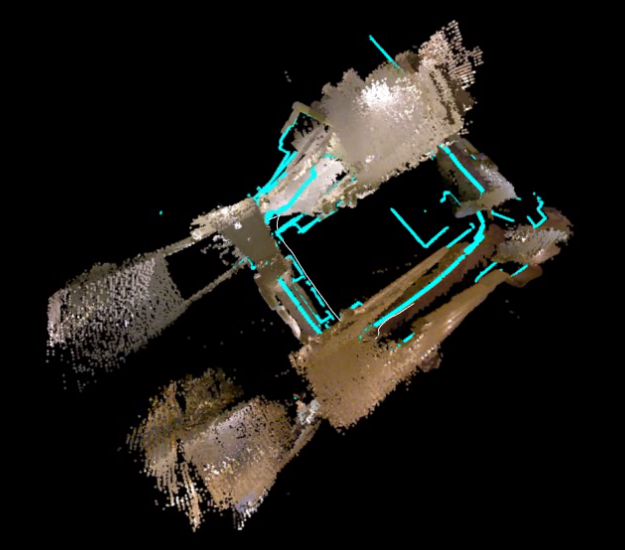
\includegraphics[width=1\textwidth]{lc_match_live_map}
	\caption{An example of an accepted loop closure hypothesis with the live robot system.}
	\label{fig:lc_match_live_map}
\end{figure}

\subsubsection{Multi Session Mapping}

\subsubsection{Navigating an Obstacle Course}



\subsubsection{Avoiding Moving Obstacles}

\begin{figure}[p]
	\centering
	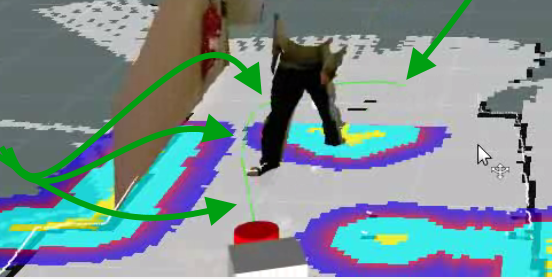
\includegraphics[width=1\textwidth]{avoiding_moving_obstacles_arrow}
	\caption{Avoiding moving obstacles with a new plan that circumnavigates the detected obstruction. In this situation, the obstacle was moving too fast for the local planner. The right leg is not yet registered as an obstacle.}
	\label{fig:avoiding_moving_obstacles}
\end{figure}

\begin{figure}
	\centering
	\begin{subfigure}[b]{0.46\textwidth}
		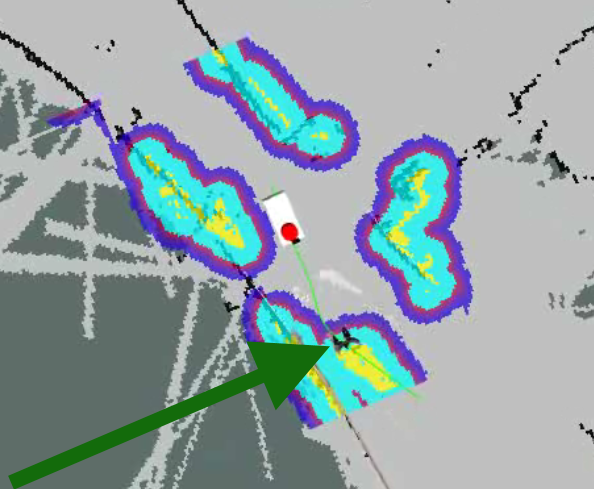
\includegraphics[width=\textwidth]{obstructed_plan_arrow}
		\caption{A person has moved into the path of the robot.}
		\label{fig:obstructed_plan}
	\end{subfigure}
	\begin{subfigure}[b]{0.472\textwidth}
		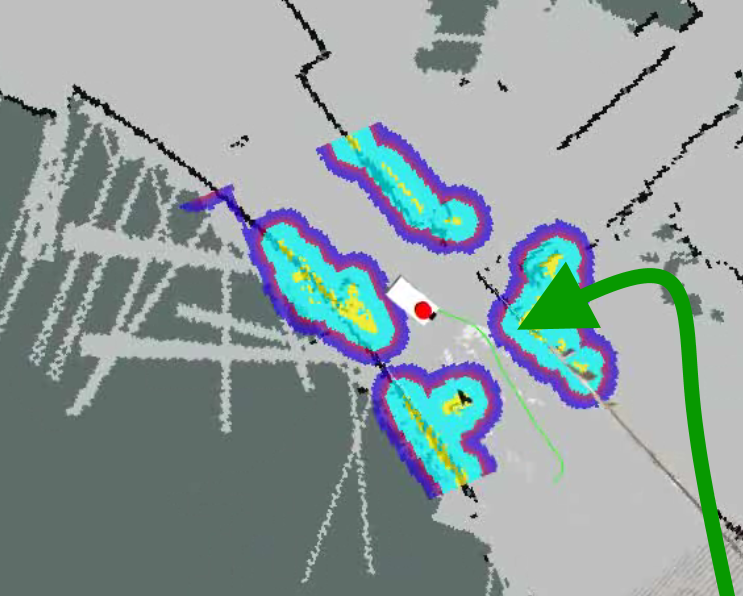
\includegraphics[width=\textwidth]{corrected_plan_arrow}
		\caption{A new path is planned, avoiding the new obstacle.}
		\label{fig:corrected_plan}
	\end{subfigure}
	\caption{Moving obstacle avoidance. The local cost map, shown as coloured spots on the occupancy grid, is based on real-time sensor data. }
\end{figure}




\section{Discussion}